\chapter{Evaluation}
\label{cha:eval}


Comparison with two of the most popular RAM-based Key-value pair databases: \textbf{memcached} and \textbf{Redis}.
Run on an ASUS X555L quadcore Intel(R) Core(TM) i5-5200U CPU @ 2.20GHz, 8gb DDR3 RAM @ 1600 MHz.

Write speed with different data sizes, etc.

256 is the limit data size of sdp messages...

As can be seen in figure XXX, the SpiNNaker Database (SpiDB) on the 4 chip board performs quite poorly against the two, running at around 7k put operations per second, compared to ... (thus slow by a factor of about 8) 


\begin{figure}
\begin{center}
	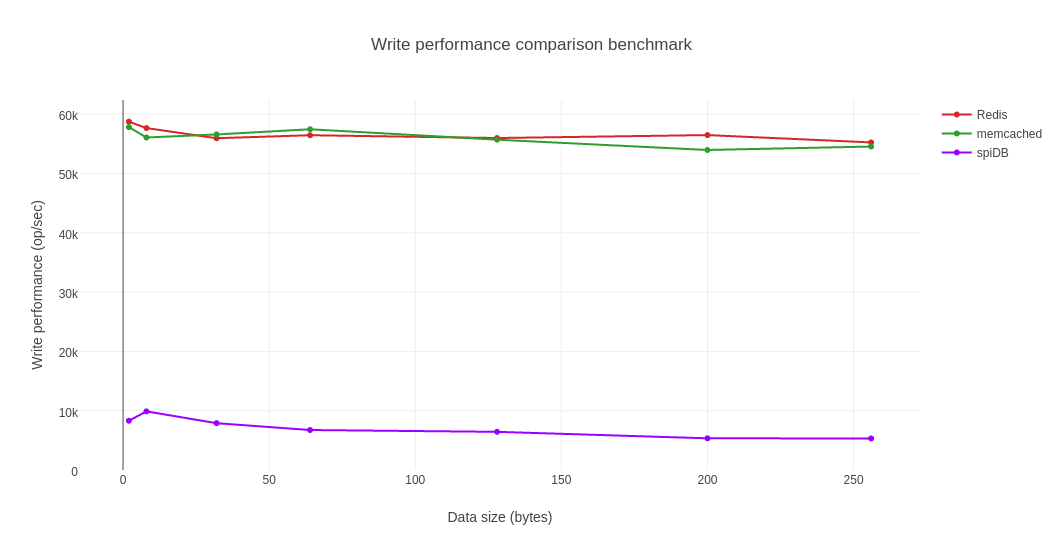
\includegraphics[width=1\textwidth, natwidth=1063, natheight=550]{images/write_performance.png}
\end{center}
\caption{Write performance benchmark}
\label{fig:die-plot}
\end{figure}

\section{Limitations}

\section{Predictions}